\documentclass{article}
\usepackage[T1]{fontenc}
\usepackage{lmodern}
\usepackage{graphicx}
\usepackage{amsmath,amssymb}
\usepackage[a4paper,margin=2cm]{geometry}
\usepackage[absolute,overlay]{textpos}
\setlength{\TPHorizModule}{1mm}
\setlength{\TPVertModule}{1mm}
\usepackage[indonesian]{babel}
\usepackage{hyperref}
\setlength{\emergencystretch}{2em}
% unit: Halaman 69

\begin{document}

% === Halaman 69 (python/native) ===

69

•

Jumlah kemungkinan matriks kunci yang bisa dibentuk:    

                 25!=15.511.210.043.330.985.984.000.000

•

Kunci enkripsi/dekripsi pada Playfair cipher disusun berbentuk 

matriks berukuran 5 x 5

•

Setiap elemen matriks adalah huruf-huruf alfabet A..Z

•

Karena ada 25 elemen matriks, dan ada 26 huruf alfabet, maka ada 

satu huruf alfabet dibuang, yaitu huruf J

% deskripsi: gambar native xref 262
\noindent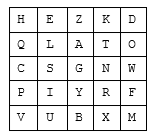
\includegraphics[width=0.85\textwidth]{../../images/python/page_069_img_01.png}

\end{document}
